\documentclass[twoside,11pt]{article}

\usepackage{aa228-jmlr2e}
\usepackage{amsmath}
\usepackage{graphicx}
\usepackage{lipsum}
\usepackage{listings}
\usepackage{url}
\usepackage{cleveref}
\usepackage{subcaption}
\usepackage{tikz}
\usetikzlibrary{arrows.meta, positioning, calc}

\begin{document}

% More details can be found here: https://aa228.stanford.edu/final-project/
\title{Automating Parametric CAD Sketch Synthesis via Sequential Decision Making}
\newcommand{\shorttitle}{Automating CAD Sketches} 

%===========================================
% Fill in your names and emails
%===========================================
\name{Christopher Luey}
\email{luey@stanford.edu}

\maketitle

\section{Goal}
Modern mechanical design teams still spend significant time translating requirement tables into parametric computer-aided design (CAD) sketches that seed downstream solid modeling. I propose to automate the early-stage sketching of planar bracket components directly from structured requirement tuples by learning from the SketchGraphs dataset ($\sim$8.8M sketches), filtering for planar brackets with $\leq$12 primitives and $\leq$3 closed profile loops \citep{Willis2021Fusion360, SketchGraphs2020}. Focusing on L- and U-shaped brackets exercises sequential decision-making tools on meaningful engineering constraints.

We have three deliverables: (i) Days 1--4: curate bracket subset from SketchGraphs filtering, report size and statistics (primitive frequencies, constraint co-occurrence, dimensional ranges), and publish preprocessing notebooks; (ii) Days 5--9: train behavior cloning baseline with ensemble uncertainty quantification, logging calibration metrics for downstream risk analysis; and (iii) Days 10--14: apply conservative Q-learning fine-tuning and evaluate with risk-sensitive metrics on held-out test sequences. Achieving these milestones will demonstrate that principled offline RL can learn sketch construction policies with quantified uncertainty \citep{Kochenderfer2022}.


\section{Decision Making}
I frame automated sketch construction as a partially observable Markov decision process (POMDP) in which each episode corresponds to building a parametric sketch that satisfies a requirement tuple $(g, c, d)$ containing desired geometry (hole pattern, flange lengths), hard constraints (mounting plane, thickness), and design intents (load directions). We frame this as a POMDP where partial observability arises naturally: at construction step $t$, the agent observes only the requirement specification and partial sketch history, but does not observe the (latent) full target sketch topology the designer intends. This captures realistic design uncertainty. The latent state $s_t$ comprises the full canonical sketch graph, including primitive embeddings, unresolved constraint slack, and metadata. The observation $o_t$ exposes the partial sketch graph available to the agent and requirement tokens.

The action space leverages SketchGraphs' taxonomy: five primitive types (line, arc, circle, point, spline) and nine constraint/dimension types (coincident, perpendicular, parallel, equal, tangent, horizontal, vertical, distance, angle) with parameter bins learned from empirical quantiles. Each action is factored into a discrete intent $a^{\text{type}}_t$ and continuous parameter vector $a^{\text{param}}_t$; the former is modeled as a categorical distribution, whereas the latter is sampled from Gaussian heads centered on dataset means with learned variance. Due to the offline nature, we approximate the environment dynamics from recorded trajectories rather than interfacing with a live CAD solver. Transitions $T(s_{t+1}\,|\,s_t, a_t)$ are approximated from offline trajectory data, treating recorded expert sequences as ground truth.

Rewards are implicit from expert demonstrations in offline RL setting. The hierarchical structure enables efficient planning: a high-level policy selects which substructure to extend (e.g., ``extend flange'') while a low-level controller chooses primitive parameters. Offline behavior cloning on filtered expert trajectories supplies the initial policy; uncertainty-aware improvement follows via conservative Q-learning with ensemble-based risk estimation.

\section{Sources of Uncertainty}
Our primary uncertainty source is epistemic: expert demonstrations exhibit multiple valid construction strategies for similar brackets (e.g., order of dimension assignment). We model this via bootstrap ensembles of graph encoders, using disagreement as a calibrated risk metric. A secondary source is specification ambiguity: requirement tuples may underspecify dimensions (fillet radii, hole clearances), which we model with learned variance heads on continuous parameters. Solver stochasticity and tolerance propagation would require live CAD kernel access beyond study's scope. We treat recorded transitions as ground truth.

During training, Monte Carlo dropout and deep ensembles yield calibrated predictive intervals; conservative Q-learning uses the lower confidence bound to penalize risky actions. At deployment, the agent selects actions using a risk-sensitive criterion $\max_a \mathbb{E}[Q(s,a)] - \lambda \sqrt{\text{Var}[Q(s,a)]}$, where $\lambda$ is tuned on validation requirements to balance aggressiveness and robustness. Evaluation will report mean performance, $95\%$ confidence intervals, and worst-case outcomes, providing a principled view of residual uncertainty.

\begin{figure}[t]
    \centering
    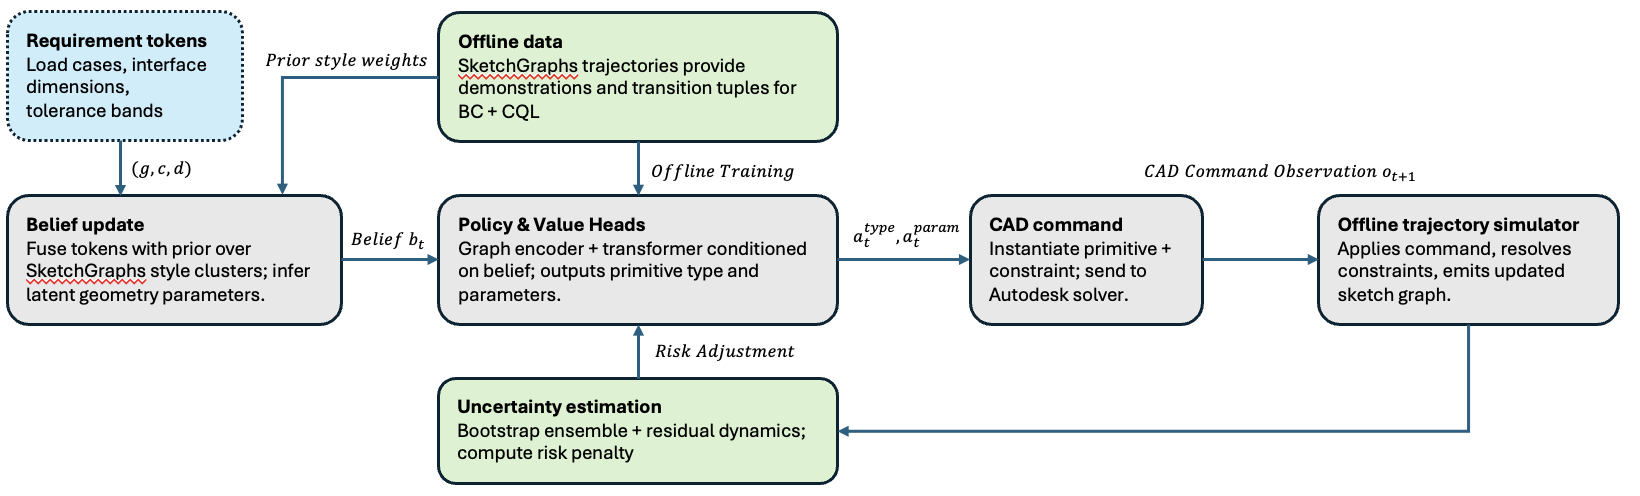
\includegraphics[width=0.9\linewidth]{flowchart.png}
    \caption{Offline decision loop with uncertainty-aware policy and trajectory simulator.}
    \label{fig:decision-flow}
\end{figure}

% References
\bibliography{references}


\end{document}

